\chapter{Implementarea Practică a Sistemului \label{implementare}}

Acest capitol detaliază procesul de realizare fizică a prototipului, selecția componentelor pentru performanța audio și soluțiile constructive pentru integrarea modulelor într-o structură compactă. De asemenea, sunt prezentate dificultățile tehnice întâmpinate în faza de punere în funcțiune și modul în care acestea au fost soluționate prin modificări la nivel hardware.

\section{Realizarea fizică și asamblarea circuitului}

Realizarea prototipului a fost efectuată pe o placă de test de tip \textit{perfboard}. Deși această metodă presupune un volum de muncă ridicat, ea a oferit flexibilitatea necesară pentru ajustări rapide în timpul fazei de prototipare.

În Figura \ref{fig:proiect_final} este prezentat ansamblul hardware finalizat, ilustrând organizarea internă a componentelor în carcasă.

\begin{figure}[htbp]
    \centering
    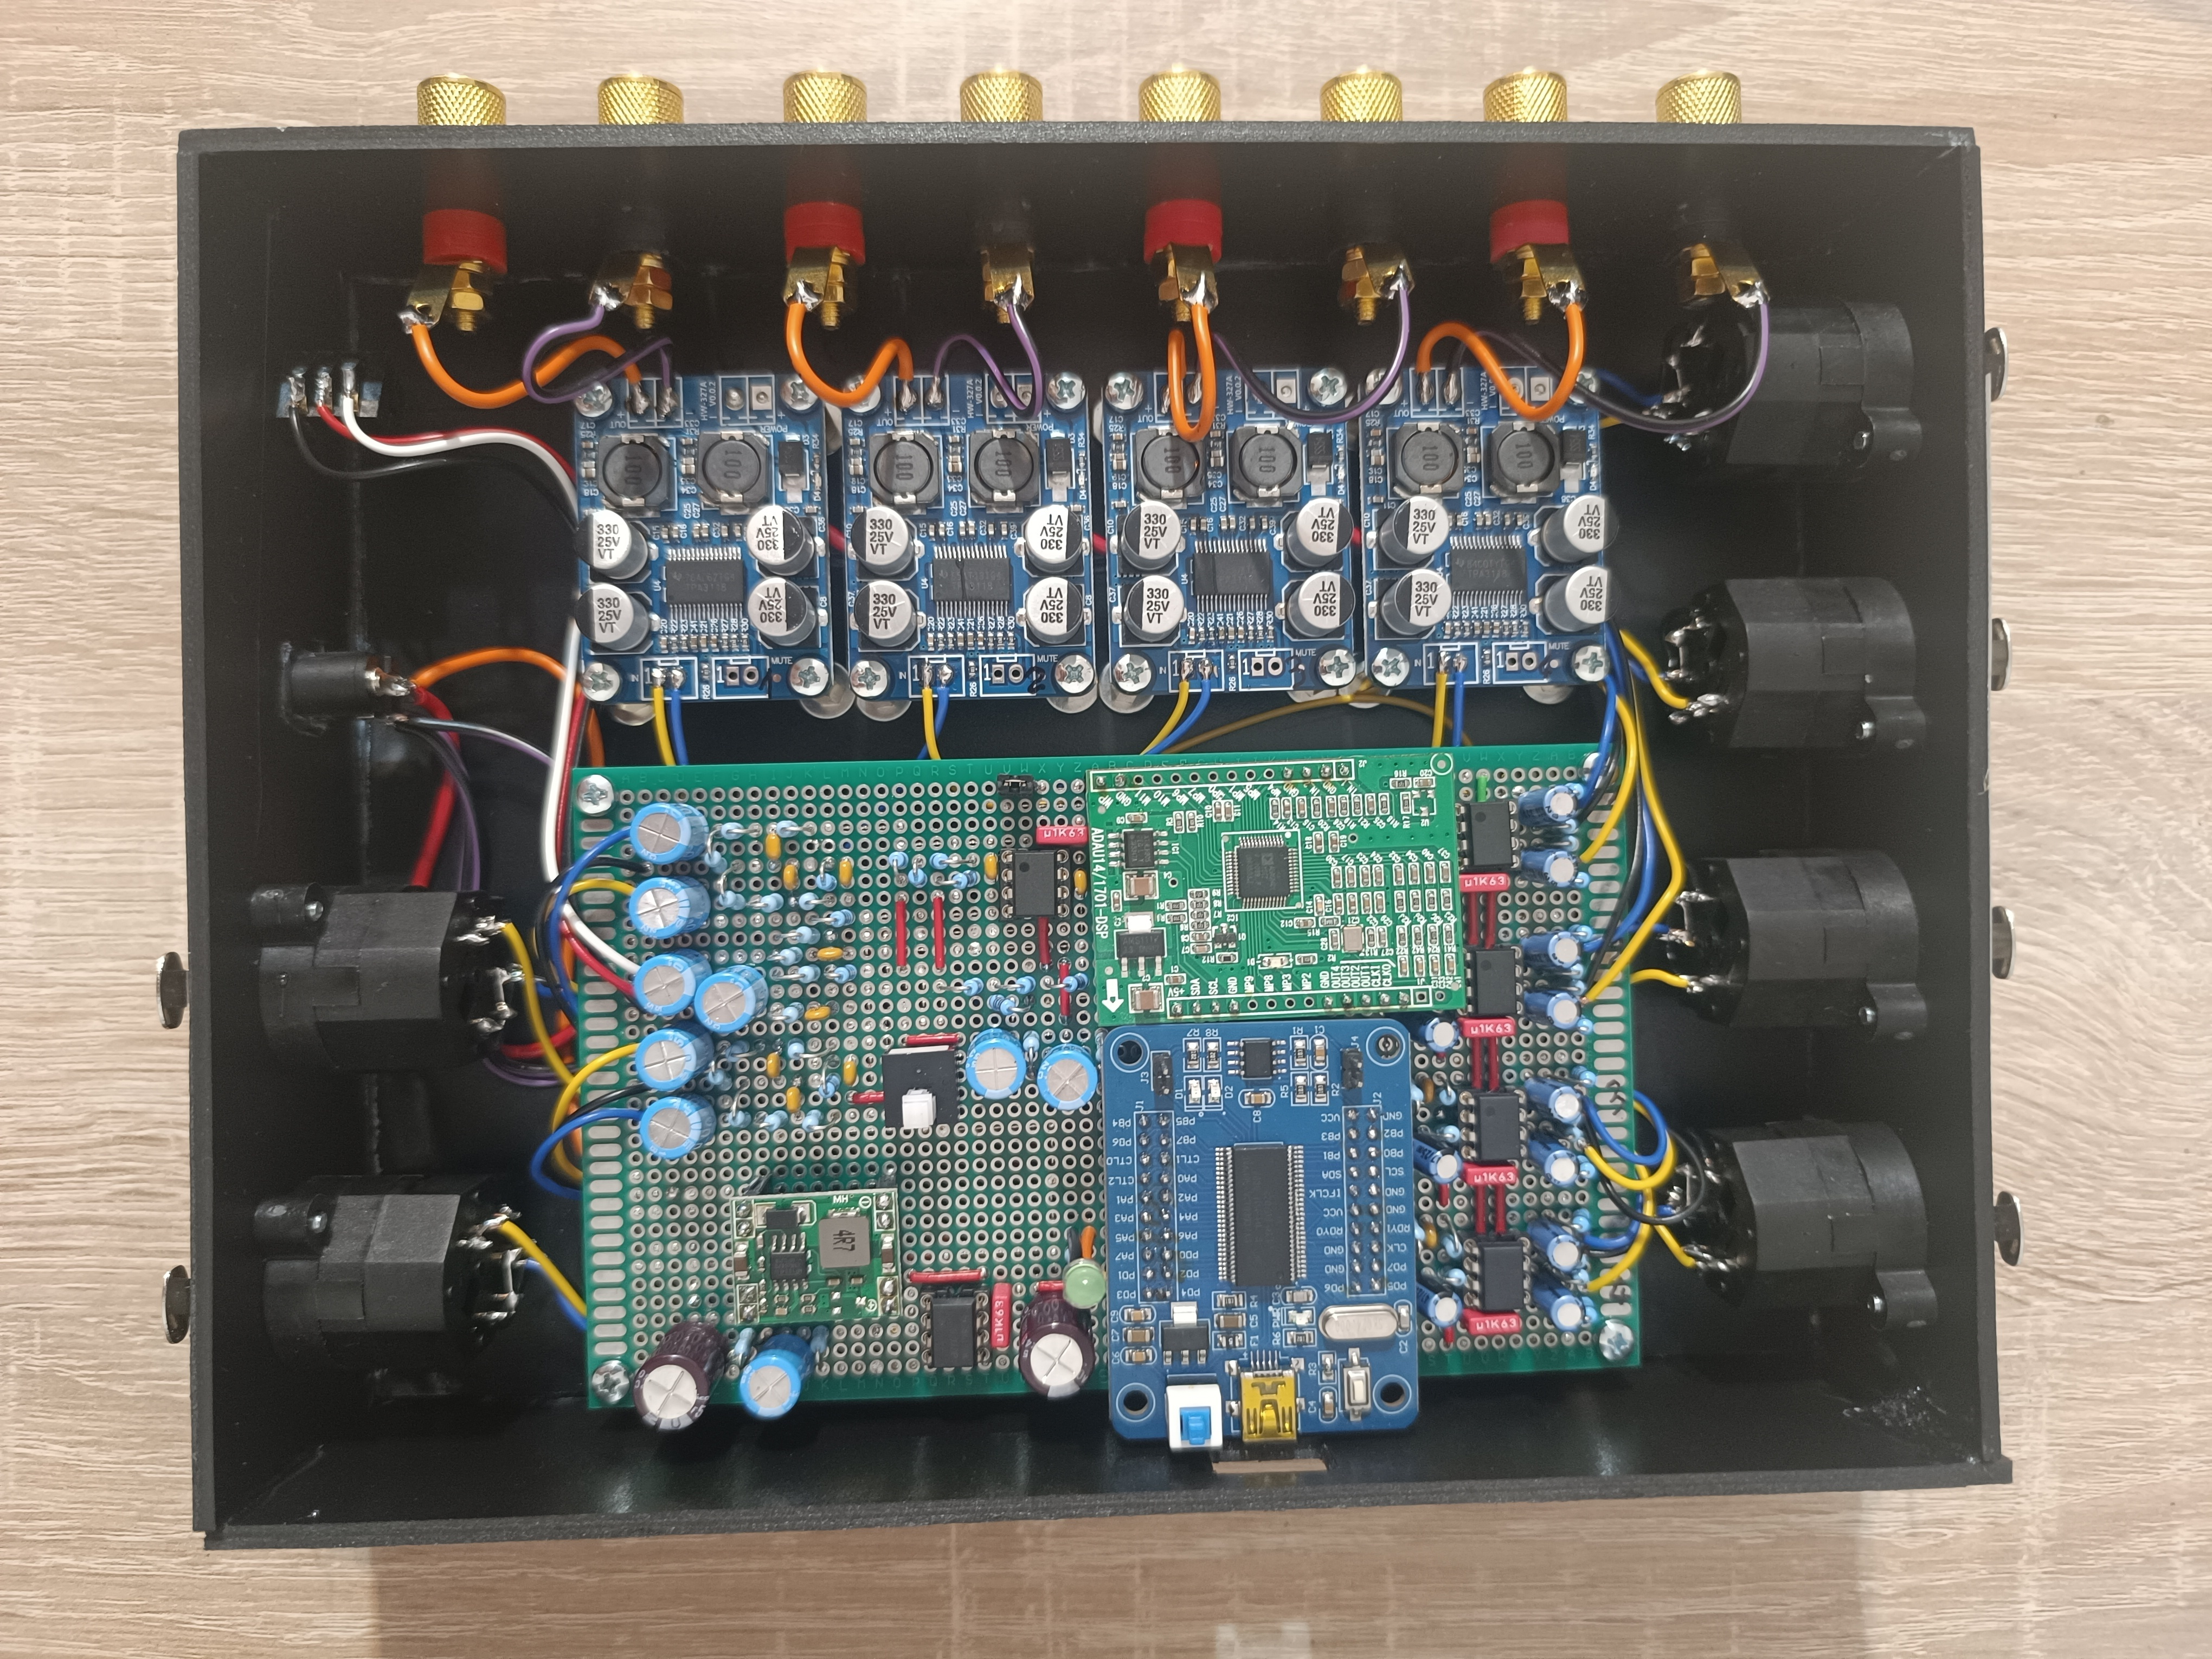
\includegraphics[width=0.9\textwidth]{figuri/DSPamp.jpg}
    \caption{Prototipul final al amplificatorului.}
    \label{fig:proiect_final}
\end{figure}

\subsection{Selecția componentelor discrete}
Calitatea audio a fost prioritară în alegerea componentelor pasive. În punctele critice ale traseului de semnal, unde a fost necesară utilizarea condensatoarelor electrolitice pentru decuplarea în curent continuu, s-au utilizat componente specializate pentru aplicații audio (ex. seria \textit{Nichicon Muse} sau echivalent). Acestea prezintă un factor de pierderi redus și o liniaritate superioară în banda audio față de componentele de uz general.

În cazul rezistențelor, s-au utilizat componente cu peliculă metalică cu toleranță de $1\%$, asigurând un nivel scăzut de zgomot termic.

\section{Integrarea modulară și construcția mecanică}

Sistemul a fost conceput pentru a fi mentenabil și extensibil, adoptând o abordare modulară pentru elementele cheie.

\subsection{Montarea componentelor active și a modulelor}
Pentru a facilita depanarea sau înlocuirea facilă a componentelor în caz de defect, s-au utilizat următoarele soluții de interconectare:
\begin{itemize}
    \item \textbf{Socluri pentru circuite integrate:} Amplificatoarele operaționale OPA2134 și TL072 au fost montate în socluri de precizie.
    \item \textbf{Barete de pini (headers):} Modulele pre-asamblate (procesorul DSP ADAU1701, programatorul USB și convertorul DC-DC LM2596) sunt conectate la placa principală prin intermediul baretelor de pini. Această configurație permite accesul rapid la module.
\end{itemize}

\subsection{Carcasa și organizarea internă}
Ansamblul hardware este găzduit într-o carcasă realizată din material plastic. Placa principală (\textit{perfboard}) și cele patru module de putere în clasa D sunt fixate rigid prin intermediul unor înălțătoare.

Conectorii sunt montați direct pe panourile carcasei, fiind conectați la circuit prin cabluri dedicate.

\section{Dificultăți tehnice și soluții de depanare}

Cea mai semnificativă problemă întâmpinată în faza de asamblare a vizat procesul de inițializare (\textit{boot-up}) al procesorului DSP ADAU1701.

În timpul testelor inițiale, s-a observat că procesorul digital de semnal refuza să pornească sau să încarce programul din memoria EEPROM externă dacă pinul \textbf{WP} (\textit{Write Protect}) era conectat permanent la masă (GND) înainte de aplicarea tensiunii de alimentare. Această condiție bloca procesul intern de pornire al DSP-ului.

Pentru a remedia această eroare de secvențiere, a fost introdus un header mic cu un jumper dedicat pentru pinul WP. Această modificare permite utilizatorului:
\begin{enumerate}
    \item Să mențină pinul WP inactiv în momentul alimentării, permițând DSP-ului să finalizeze secvența de boot;
    \item Să dezactiveze protecția la scriere (prin punerea jumper-ului la GND) abia după ce sistemul a pornit corect;
    \item Să configureze pinul doar atunci când este necesară programarea efectivă a memoriei.
\end{enumerate}

Această soluție a asigurat fiabilitatea pornirii sistemului și a oferit un mecanism hardware simplu de control pentru accesul la memoria non-volatilă.
